\documentclass[11pt,a4paper]{article}
\usepackage[T1]{fontenc}
\usepackage{amsmath,amssymb,graphicx,caption}
\usepackage[margin=22mm]{geometry}

\renewcommand{\theequation}{S\arabic{equation}}
\renewcommand{\thefigure}{S\arabic{figure}}

\title{Supplementary Material for\\
RAPTOR: Resource-Aware Physics-Token Operator with Residual Local Adaptation
for Aerodynamic Field Reconstruction}
\author{}
\date{}

\begin{document}
\maketitle
\vspace{-2em}

\section*{Illustrative AirfRANS pressure-error cases}

Figure~\ref{fig:airfrans_pressure_cases} preserves the two seed-42
pressure-divided-by-density (\(p/\rho\)) examples formerly shown in the main
manuscript. The upper row is from Reynolds-number extrapolation and compares
RAPTOR with Transolver-Tiny; the lower row is from angle-of-attack (AoA)
extrapolation and compares RAPTOR with LinearNO-Tiny. The comparator in each
row ranks second by the four-variable macro relative \(L_2\) error in the
corresponding seed-42 experiment.

Each case contains \(N=4096\) sampled nodes. For model \(a\), test case
\(q\), and the \(p/\rho\) channel, define the sample-level error and pooled
test-set error as
\begin{equation}
e_{q,p}^{(a)}
=
\frac{\|\widehat{\mathbf Y}_{q,p}^{(a)}-\mathbf Y_{q,p}\|_2}
{\|\mathbf Y_{q,p}\|_2+10^{-12}},
\qquad
\varepsilon_p^{(a)}
=
\frac{\sqrt{\sum_{q=1}^{M}
\|\widehat{\mathbf Y}_{q,p}^{(a)}-\mathbf Y_{q,p}\|_2^2}}
{\sqrt{\sum_{q=1}^{M}\|\mathbf Y_{q,p}\|_2^2}+10^{-12}}.
\label{eq:supp_pressure_errors}
\end{equation}
Here \(M=200\) for Reynolds-number extrapolation and \(M=196\) for AoA
extrapolation. Let \(R\) denote RAPTOR and \(b\) the comparator in the same
row. The displayed test case minimizes the distance between its paired
pressure improvement and the pooled test-set pressure improvement:
\begin{equation}
\Delta_p^{\mathrm{test}}
=1-\frac{\varepsilon_p^{(R)}}{\varepsilon_p^{(b)}},
\qquad
\Delta_{q,p}
=1-\frac{e_{q,p}^{(R)}}{e_{q,p}^{(b)}},
\qquad
q^*=\operatorname*{arg\,min}_{q}
\left|\Delta_{q,p}-\Delta_p^{\mathrm{test}}\right|.
\label{eq:supp_case_selection}
\end{equation}
The selected test indices are 165 and 142 for Reynolds-number and AoA
extrapolation, respectively. The pooled/selected improvements are
\(4.84\%/4.97\%\) and \(4.63\%/4.17\%\), respectively. On these selected
cases, RAPTOR changes the sample-level \(p/\rho\) relative \(L_2\) error
from 0.277 to 0.263 and from 0.274 to 0.262, respectively. All metrics
use the sampled nodes; percentile normalization affects only the
displayed absolute-error colors.

\begin{center}
    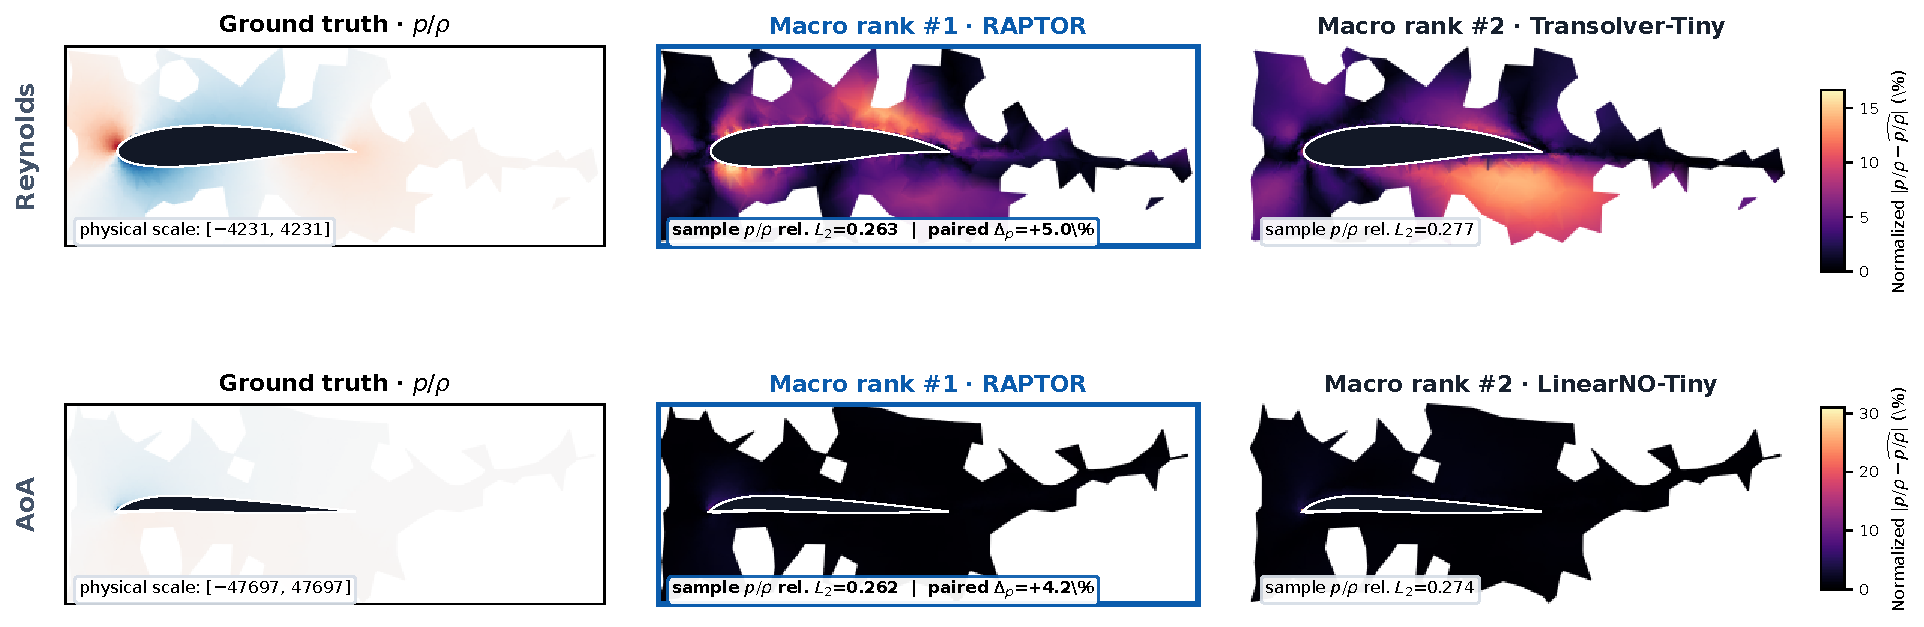
\includegraphics[width=\linewidth,height=0.50\textheight,keepaspectratio]
    {figs/Fig2.pdf}
    \captionof{figure}{Seed-42 AirfRANS \(p/\rho\) ground truth and
    normalized absolute-error maps. Reynolds-number test index 165
    (upper row) compares RAPTOR with Transolver-Tiny; AoA test index
    142 (lower row) compares RAPTOR with LinearNO-Tiny. The cases are
    selected by Equation~\eqref{eq:supp_case_selection}, not by the
    largest visual or sample-level improvement. These seed-42 maps are
    illustrative; they do not establish cross-seed stability or a
    systematic physical correction mechanism.}
    \label{fig:airfrans_pressure_cases}
\end{center}

\end{document}
